% !TEX root = ../FundationsDataScience.tex

\chapter{Non-smooth Convex Optimization}
\label{chap-conv-duality}

The main references for this chapter are~\cite{chambolle2010introduction,chambolle2016introduction,boyd2004convex}, see also~\cite{parikh2014proximal,boyd2011distributed,beck2014introduction}. 

We consider a general convex optimization problem
\eql{\label{eq-general-pbm} 
	\umin{x \in \Hh} f(x)
}
where $\Hh=\RR^p$ is a finite dimensional Hilbertian (i.e. Euclidean) space, 
and try to devise ``cheap'' algorithms with a low computational cost per iterations. The class of algorithms considered are first order, i.e. they make use of gradient information. 


%%%%%%%%%%%%%%%%%%%%%%%%%%%%%%%%%%%%%%%%%%%%%%%%%%%%%%%%%%%%%%%%%%%%%%%%%%%%%%%%%%
%%%%%%%%%%%%%%%%%%%%%%%%%%%%%%%%%%%%%%%%%%%%%%%%%%%%%%%%%%%%%%%%%%%%%%%%%%%%%%%%%%
%%%%%%%%%%%%%%%%%%%%%%%%%%%%%%%%%%%%%%%%%%%%%%%%%%%%%%%%%%%%%%%%%%%%%%%%%%%%%%%%%%
\section{Descent Methods}
\label{sec-grad-descent}

We have already encountered the gradient descent method informally in Section~\ref{} for the regularization of inverse problem. We now give a detailed analysis of the method.

%%%%%%%%%%%%%%%%%%%%%%%%%%%%%%%%%%%%%%%%%%%%%%%%%%%%%%%%%%%%%%%%%%%%%%%%%%%%%%%%%%
\subsection{Gradient Descent}

The optimization program~\eqref{eq-ip-tv-eps} is an example of unconstrained convex optimization of the form~\eqref{eq-general-pbm} where $f : \Hh \rightarrow \RR$ is a $\Cc^1$ function with Lipschitz gradient (so-called ``smooth'' function). Recall that the gradient $\nabla f : \Hh \mapsto \Hh$ of this functional (not to be confound with the discretized gradient $\nabla x \in \Hh$ of $f$) is defined by the following first order relation
\eq{
	f(x+r) = f(x) + \dotp{f}{r}_{\Hh} + O(\norm{r}_{\Hh}^2)
}
where we used $O(\norm{r}_{\Hh}^2)$ in place of $o(\norm{r}_{\Hh})$ (for differentiable function) because we assume here $f$ is of class $\Cc^1$ (i.e. the gradient is continuous). Section~\ref{eq-example-grad} shows typical examples of gradient computation.

For such a function, the gradient descent algorithm is defined as
\eql{\label{eq-grad-desc}
	\iit{x} \eqdef \it{x} - \tau_\ell \nabla f( \it{x} ), 
}
where the step size $\tau_\ell>0$ should be small enough to guarantee convergence, but large enough for this algorithm to be fast.


%%%%%%%%%%%%%%%%%%%%%%%%%%%%%%%%%%%%%%%%%%%%%%%%
\subsection{Sub-gradient Descent}

The gradient descent~\eqref{eq-grad-desc} cannot be applied on a non-smooth function $f$. One can use in place of a gradient a sub-gradient, which defines the sub-gradient descent
\eql{\label{eq-subgrad-desc}
	\iit{x} \eqdef \it{x} - \tau_\ell \it{g}
	\qwhereq
	\it{g} \in \partial f( \it{x} ).
}
The main issue with this scheme is that to ensure convergence, the iterate should go to zero. One can easily convince oneself why by looking at the iterates on a function $f(x)=|x|$.

\begin{thm}
	If $\sum_{\ell} \tau_\ell=+\infty$ and $\sum_{\ell} \tau_\ell^2 < +\infty$, then $\it{x}$ converges to a minimizer of $f$. 
\end{thm}

%%%%%%%%%%%%%%%%%%%%%%%%%%%%%%%%%%%%%%%%%%%%%%%%%%%%%%%%%%%%%%%%%%%%%%%%%%%%%%%%%%
\subsection{Projected Gradient Descent}
\label{sec-proj-grad}

We consider a generic constraint optimization problem as
\eql{\label{eq-constr}
	\umin{x \in \Cc} f(x) 
} 
where $\Cc \subset \RR^S$ is a closed convex set and $f : \RR^S \rightarrow \RR$ is a smooth convex function (at least of class $\Cc^1$). 

The gradient descent algorithm~\eqref{eq-grad-desc} is generalized to solve a constrained problem using the projected gradient descent 
\eql{\label{eq-proj-grad-desc}
	\iit{x} \eqdef \Proj_\Cc \pa{ \it{x} - \tau_\ell \nabla f( \it{x} ) }, 
}
where $\Proj_\Cc$ is the orthogonal projector on $\Cc$
\eq{
	\Proj_\Cc(x) = \uargmin{x' \in \Cc} \norm{x-x'}
}
which is always uniquely defined because $\Cc$ is closed and convex.
%
The following proposition shows that all the convergence properties of the classical gradient descent caries over to this projected algorithm.

\begin{thm}\label{thm-proj-grad}
	Theorems~\ref{thm-gradsec-strong-conv} and~\ref{thm-gradsec-non-strong-conv} still holds when replacing iterations~\eqref{eq-grad-desc} by~\eqref{eq-proj-grad-desc}.
\end{thm}

\begin{proof}
	The proof of Theorem~\ref{thm-gradsec-strong-conv} extends because the projector is contractant, 
	$\norm{\Proj_\Cc(x)-\Proj_\Cc(x')} \leq \norm{x-x'}$ so that the strict contraction properties of the gradient descent is maintained by this projection.   
\end{proof}

The main bottleneck that often prevents to use~\eqref{eq-proj-grad-desc} is that the projector is often complicated to compute. We are however lucky since for $\ell^1$ mininization, one can apply in a straightforward manner this method. 




%%%%%%%%%%%%%%%%%%%%%%%%%%%%%%%%%%%%%%%%%%%%%%%%%%%%%%%%%%%%%%%%%%%%%%%%%%%%%%%%%%
%%%%%%%%%%%%%%%%%%%%%%%%%%%%%%%%%%%%%%%%%%%%%%%%%%%%%%%%%%%%%%%%%%%%%%%%%%%%%%%%%%
%%%%%%%%%%%%%%%%%%%%%%%%%%%%%%%%%%%%%%%%%%%%%%%%%%%%%%%%%%%%%%%%%%%%%%%%%%%%%%%%%%
\section{Proximal Algorithm}

For non-smooth functions $f$, it is not possible to perform an ``explicit'' gradient descent step because the gradient is not even defined. One thus needs to replace this ``explicit''  step by an ``implicit'' one, which is possible even if $f$ is non-smooth.


%%%%%%%%%%%%%%%%%%%%%%%%%%%%%%%%%%%%%%%%%%%%%%%%
\subsection{Proximal Map }

The implicit stepping of amplitude $\tau>0$ is defined as 
\eql{\label{eq-defn-proximal}
	\foralls x, \quad
	\Prox_{\tau f}(x) \eqdef \uargmin{x'} \frac{1}{2}\norm{x-x'}^2 + f(x').
}
It amounts to minimize function $f$ locally around $x$, in a ball of radius controlled by $\tau$.
%
This the involved function $\frac{1}{2}\norm{x-\cdot}^2 + f$ is strongly convex, this operator $\Prox_{\tau f}$ is well defined and single-valued. 

When $f=\iota_\Cc$ is an indicator, the proximal map boils down to a projection $\Prox_{\iota_\Cc}=\Proj_{\Cc}$, it is thus in some sense a generalization of the projection to arbitrary function. And can also be interpreted as a projector on a level set of $f$.  An interesting feature of the proximal map is that it is a contraction, thus generalizing the well-known property of projectors.

\begin{prop}
	One has $\norm{ \prox_{f}(x)-\prox_{f}(y) } \leq \norm{x-y}$.
\end{prop}



\begin{figure}
\centering
%%
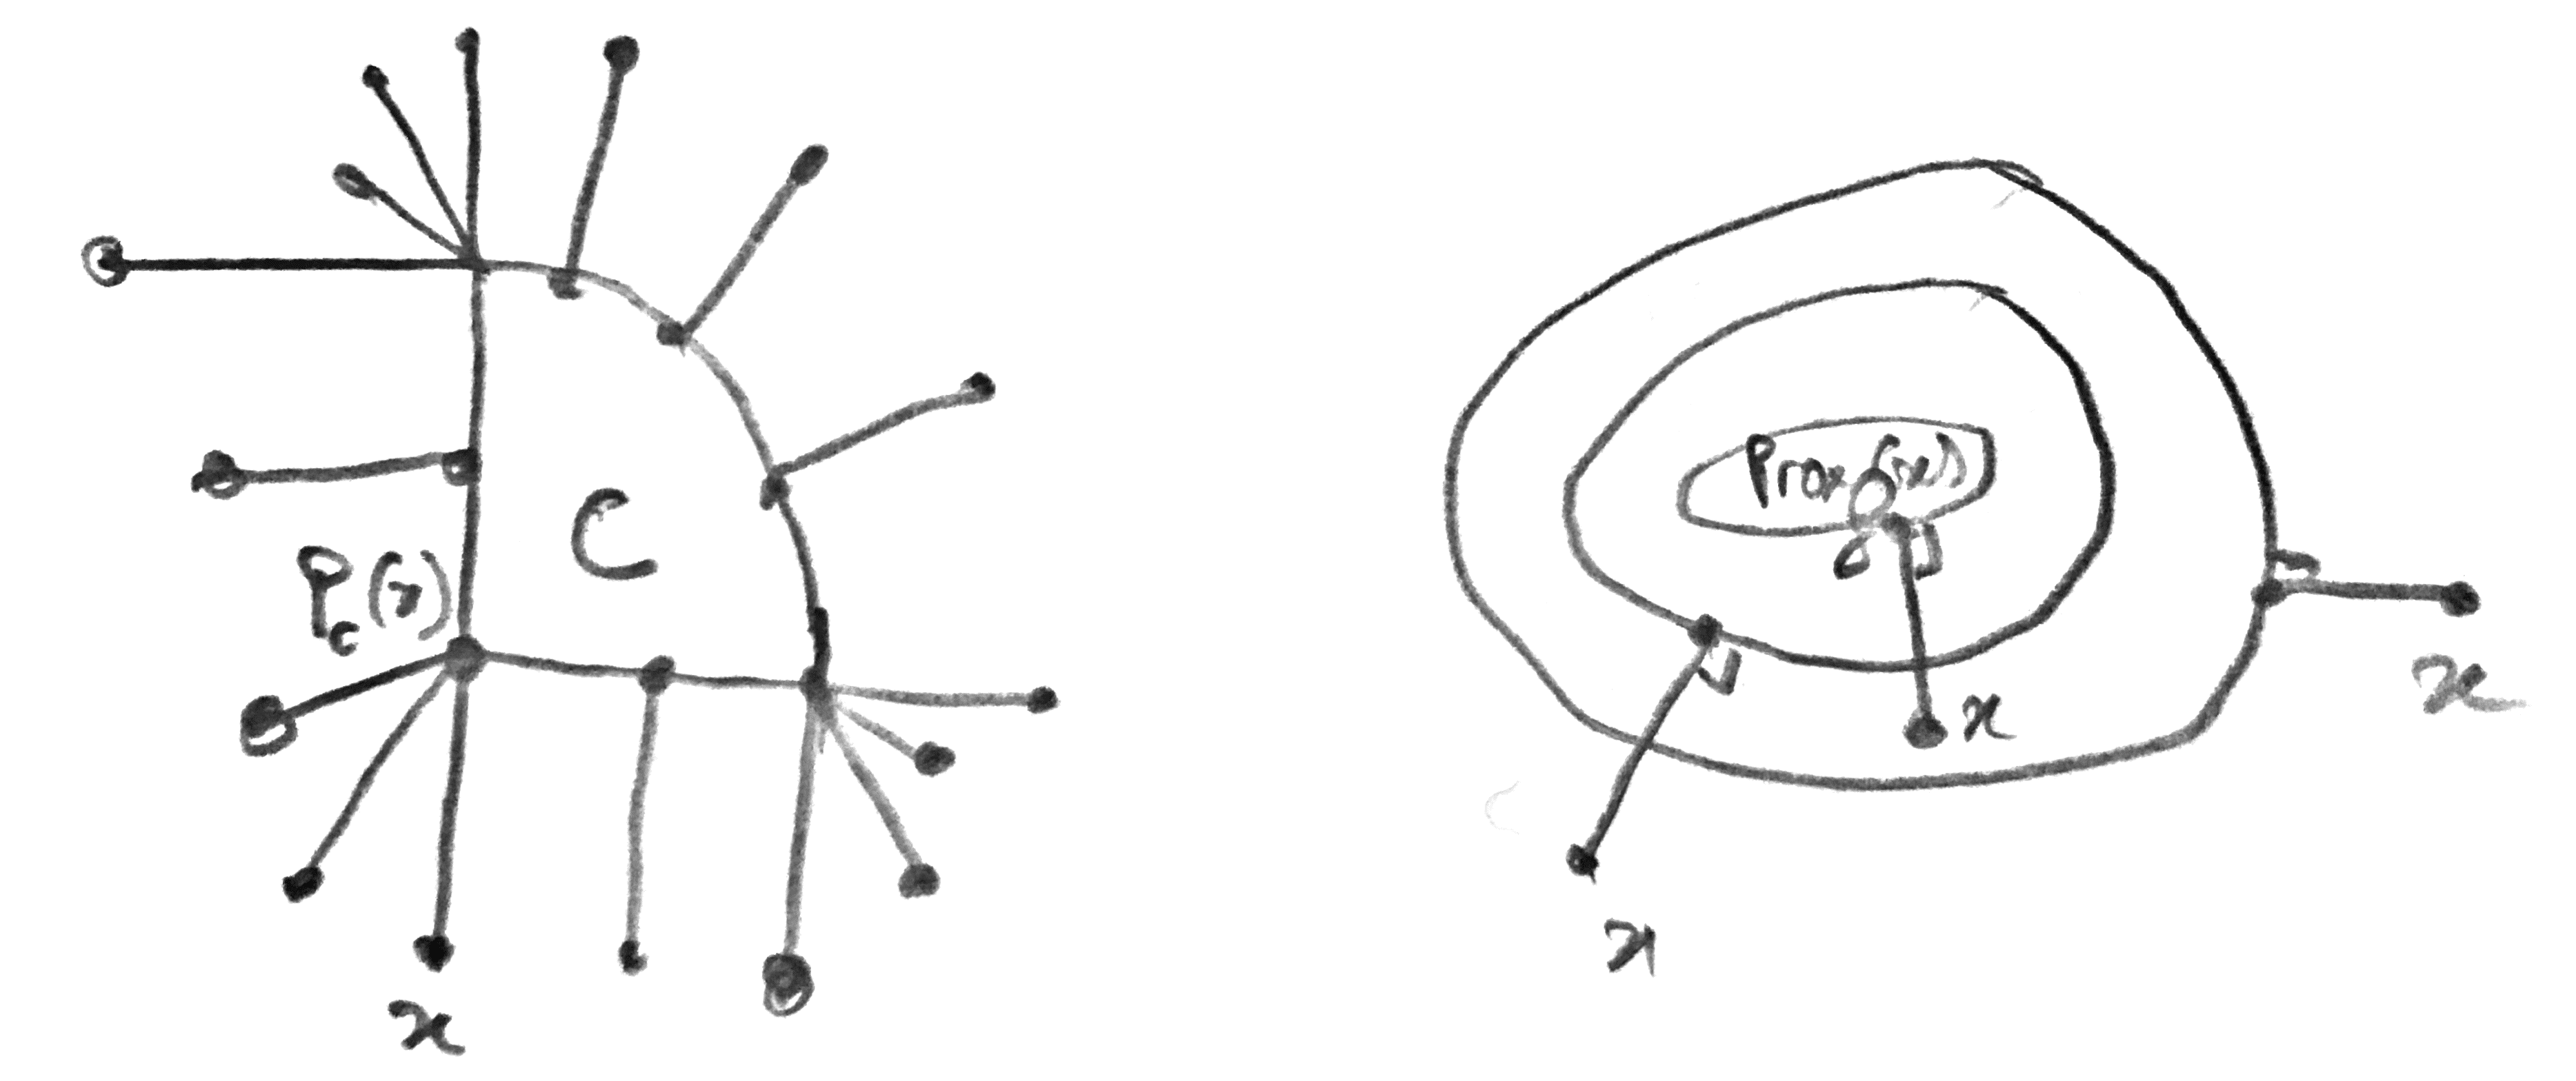
\includegraphics[width=.6\linewidth]{convexity/prox-proj}
%%
\caption{\label{fig-prox-proj}
Proximal map and projection map.}
\end{figure}


%%%
\paragraph{Examples}

The following proposition states a few simples examples.

\begin{prop}
One has
\eql{\label{eq-prox-l2-l1}
	\Prox_{\frac{\tau}{2} \norm{\cdot}^2}(x) =  \frac{x}{1+\tau}, 
	\qandq
	\Prox_{\tau \norm{\cdot}_1} = \Ss_\tau^1(x), 
}
where the soft-thresholding is defined as
\eq{
	\Ss_\tau^1(x) \eqdef ( S_\tau(x_i) )_{i=1}^p \qwhereq
	S_\tau(r) \eqdef \sign(r) (|r|-\la)_+,
}
(see also~\eqref{eq-soft-thresh}). For $A \in \RR^{P \times N}$, one has
\eql{\label{eq-prox-quad}
	\Prox_{\frac{\tau}{2}\norm{A \cdot-y}^2}(x) = (\Id_N + \tau A^* A)^{-1} ( x + \tau A^* y ).
	%= (\Id_{P} +\tau A^*A)^{-1} A^*	=  A^* (\Id_N + \tau AA^*)^{-1} 
}
\end{prop}
\begin{proof}
	The proximal map of $\norm{\cdot}_1$ was derived in Proposition~\ref{prop-equiv-sparse-thresh}.
	%
	For the quadratic case
	\eq{
		z = \Prox_{\frac{\tau}{2}\norm{A \cdot-y}^2}(x) 
		\quad\Leftrightarrow\quad 
		z-x + \tau A^*( A z - y ) = 0
		\quad\Leftrightarrow\quad
		(\Id_N + \tau A^* A) z = x + \tau A^* y.
	}
\end{proof}


Note that in some case, the proximal map of a non-convex function is well defined, for instance
$\Prox_{\tau \norm{\cdot}_0}$ is the hard thresholding associated to the threshold $\sqrt{2\tau}$, see Proposition~\ref{prop-equiv-sparse-thresh}.


%%%%%%%%%%%%%%%%%%%%%%%%%%%%%%%%%%%%%%%%%%
\subsection{Basic Properties}

We recap some useful proximal-calculus.

\begin{prop}
One has
\eq{
	\Prox_{f+\dotp{y}{\cdot}} = y + \Prox_{f}, \quad
	\Prox_{f(\cdot-y)} = y + \Prox_{f}(\cdot-y).
}
If $f(x)=\sum_{k=1}^K f(x_k)$ for $x=(x_1,\ldots,x_K)$ is separable, then
\eql{\label{eq-prox-separable}
	\Prox_{\tau f}(x) = ( \Prox_{\tau f_k}(x_k) )_{k=1}^K.
}
\end{prop}
\begin{proof}
	One has
	\eq{
		z = \Prox_{f+\dotp{y}{\cdot}}(x) 
		\quad\Leftrightarrow\quad 0 \in x-z + (\partial f(x)+y) 
		\quad\Leftrightarrow\quad 0 \in x-(z-y) + \partial f(x) 
	}
	which is the optimality condition for $z-y = \Prox_{f}(x)$.
	
	
	One has
	\eq{
		z = \Prox_{f(\cdot-y)}(x)
		\quad\Leftrightarrow\quad 0 \in x-z + \la \partial f(x-y)
		\quad\Leftrightarrow\quad 0 \in x'-(z-y) + \partial f(x') 
	}
	where we defined $x' \eqdef x-y$, and this is the optimality condition for $z-y = \Prox_{f}(x')$
\end{proof}

The following proposition is very useful.

\begin{prop}\label{prop-prox-tightframe}
	If $A \in \RR^{P \times N}$ is a tight frame, i.e. $AA^*=\Id_P$, then 
	\eq{
		\Prox_{f \circ A} = A^* \circ \Prox_{f} \circ A + \Id_N - A^* A.
	}
	In particular, if $A$ is orthogonal, then $\Prox_{f \circ A} = A^* \circ \Prox_{f} \circ A$.
\end{prop}


%%%%%%%%%%%%%%%%%%%%%%%%%%%%%%%%%%%%%%%%%%
\subsection{Related Concepts}

%%%
\paragraph{Link with sub-differential.}

For a set-valued map $U : \Hh \hookrightarrow \Gg$, we define the inverse set-valued map $U^{-1} : \Gg \hookrightarrow \Hh$ by 
\eql{\label{eq-inv-setvalued}
	h \in U^{-1}(g) 
	\quad\Longleftrightarrow\quad
	g \in U(h) 
} 
\todo{ add picture }
The following proposition shows that the proximal map is related to a regularized inverse of the sub-differential.


\begin{prop}
	One has $\Prox_{\tau f} = (\Id+\tau\partial f)^{-1}$.
\end{prop}
\begin{proof}
One has the following equivalence
\eq{
	z = \Prox_{\tau f}(x) 
	\Leftrightarrow
	0 \in z-x+\tau\partial f(z)
	\Leftrightarrow
	x \in (\Id+\tau\partial f)(z)
	\Leftrightarrow
	z = (\Id+\tau\partial f)^{-1}(x)
}	
where for the last equivalence, we have replace ``$\in$'' by ``$=$'' because the proximal map is single valued.
\end{proof}

The proximal operator is hence often referred to the ``resolvent'' $\Prox_{\tau f} = (\Id+\tau\partial f)^{-1}$ of the maximal monotone operator $\partial f$. 

%%%%
\paragraph{Link with duality.}

One has the following fundamental relation between the proximal operator of a function and of its Legendre-Fenchel transform

\begin{thm}[Moreau decomposition]
	One has
	\eq{
		\Prox_{\tau f} = \Id - \tau \Prox_{f^* / \tau}( \cdot/\tau ).
	}
\end{thm}

This theorem shows that the proximal operator of $f$ is simple to compute if and only the proximal operator of $f^*$ is also simple. 
%
As a particular instantiation, since according to , one can re-write the soft thresholding as follow
\eq{
	\Prox_{\tau \norm{\cdot}_1}(x) =  x - \tau \Proj_{\norm{\cdot}_\infty \leq 1}( x/\tau )
	 =  x -  \Proj_{\norm{\cdot}_\infty \leq \tau}( x )
	 \qwhereq
	 \Proj_{\norm{\cdot}_\infty \leq \tau}( x ) = \min(\max(x,-\tau),\tau).
}

In the special case where $f=\iota_{\Cc}$ where $\Cc$ is a closed convex cone, then
\eql{\label{eq-polar-cone}
	(\iota_{\Cc})^* = \iota_{\Cc^\circ} 
	\qwhereq
	\Cc^\circ \eqdef \enscond{y}{ \foralls x \in \Cc, \dotp{x}{y} \leq 0 } 
}	
and $\Cc^\circ$ is the so-called polar cone. Cones are fundament object in convex optimization because they are invariant by duality, in the sense of~\eqref{eq-polar-cone} (if $\Cc$ is not a cone, its Legendre transform would not be an indicator).
%
Using~\eqref{eq-polar-cone}, one obtains the celebrated Moreau polar decomposition
\eq{
	x = \Proj_{\Cc}(x) +^\bot \Proj_{\Cc^\circ}(x)
} 
where ``$+^\bot$'' denotes an orthogonal sum (the terms in the sum are mutually orthogonal). \todo{add drawing}
%
In the case where $\Cc=V$ is a linear space, this corresponds to the usual decomposition $\RR^p = V \oplus^\bot V^\bot$. 

%%%%
\paragraph{Link with Moreau-Yosida regularization.}

The following proposition shows that the proximal operator can be interpreted as performing a gradient descent step on the Moreau-Yosida smoothed version $f_\mu$ of $f$, defined in~\eqref{eq-moreau-yosida}.

\begin{prop}
	One has
	\eq{
		\Prox_{\mu f} = \Id - \mu \nabla f_\mu.
	}
\end{prop}


%%%%%%%%%%%%%%%%%%%%%%%%%%%%%%%%%%%%%%%%%%%%%%%%%%%%%%%%%%%%%%%%%%%%%%%%%%%%%%%%%%
%%%%%%%%%%%%%%%%%%%%%%%%%%%%%%%%%%%%%%%%%%%%%%%%%%%%%%%%%%%%%%%%%%%%%%%%%%%%%%%%%%
%%%%%%%%%%%%%%%%%%%%%%%%%%%%%%%%%%%%%%%%%%%%%%%%%%%%%%%%%%%%%%%%%%%%%%%%%%%%%%%%%%
\section{Primal Algorithms}

We now describe some important algorithm which assumes some structure (a so-called ``splitting'') of the minimized functional to be able to apply proximal maps on sub-functions.
%
Note that there is obviously many ways to split or structure a given initial problem, so there are many non-equivalent ways to apply a given proximal-based method to solve the problem. Finding the ``best'' way to split a problem is a bit like black magic, and there is no definite answer.
%
Also all there algorithm comes with step size and related parameters, and there is no obvious way to tune these parameters automatically (although some insight might be gained by studying convergence rate).

%%%%%%%%%%%%%%%%%%%%%%%%%%%%%%%%%%%%%%%%%%%%%%%%
\subsection{Proximal Point Algorithm}

One has the following equivalence 
\begin{align}\label{eq-proxpoint-fix}
	x^\star \in \argmin f
	&\quad\Leftrightarrow\quad
	0 \in \partial f(x^\star)
	\quad\Leftrightarrow\quad
	x^\star \in (\Id+\tau \partial f)(x^\star) \\
	&\quad\Leftrightarrow\quad
	x^\star = (\Id+\tau \partial f)^{-1}(x^\star) = \Prox_{\tau f}(x^\star).
\end{align}
This shows that being a minimizer of $f$ is equivalent to being a fixed point of $\Prox_{\tau f}$.
%
This suggest the following fixed point iterations, which are called the proximal point algorithm 
\eql{\label{eq-proximal-point}
	\iit{x} \eqdef \Prox_{\tau_\ell f}(\it{x}).
}
On contrast to the gradient descent fixed point scheme, the proximal point method is converging for any sequence of steps.

\begin{thm}
	If $0<\tau_{\min} \leq \tau_\ell \leq \ga_{\max} < +\infty$, then $\it{x} \rightarrow x^\star$ a minimizer of $f$.
\end{thm}

This implicit step~\eqref{eq-proximal-point} should be compared with a gradient descent step~\eqref{eq-grad-desc}
\eq{
	\iit{x} \eqdef (\Id+\tau_\ell \nabla f)(\it{x}).
}
One sees that the implicit resolvent $(\Id-\tau_\ell \partial f)^{-1}$ replaces the explicit step $\Id+\tau_\ell \nabla f$. For small $\tau_\ell$ and smooth $f$, they are equivalent at first order. But the implicit step is well defined even for non-smooth function, and the scheme (the proximal point) is always convergent (whereas the explicit step size should be small enough for the gradient descent to converge). This is inline with the general idea the implicit stepping (e.g. implicit Euler for integrating ODE, which is very similar to the proximal point method) is more stable. Of course, the drawback is that explicit step are very easy to implement whereas in general proximal map are hard to solve (most of the time as hard as solving the initial problem).


%%%%%%%%%%%%%%%%%%%%%%%%%%%%%%%%%%%%%%%%%%%%%%%%
\subsection{Forward-Backward}
\label{sec-fb}

It is in general impossible to compute $\Prox_{\ga f}$ so that the proximal point algorithm is not implementable.
%
In oder to derive more practical algorithms, it is important to restrict the class of considered function, by imposing some structure on the function to be minimized. We consider functions of the form
\eql{\label{eq-fb-split}
	\umin{x} \Ee(x) \eqdef f(x) + g(x)
}
where $g \in \Ga_0(\Hh)$ can be an arbitrary, but $f$ needs to be smooth.

One can modify the fixe point derivation~\eqref{eq-proxpoint-fix} to account for this special structure
\begin{align*}
 	x^\star \in \argmin f + g
	& \quad\Leftrightarrow\quad
	0 \in \nabla f(x^\star) + \partial g(x^\star) 
	\quad\Leftrightarrow\quad
	x^\star - \tau \nabla f(x^\star) \in (\Id+\tau \partial g)(x^\star) \\
	& \quad\Leftrightarrow\quad
	x^\star = ( \Id + \tau \partial g )^{-1} \circ ( \Id - \tau \nabla f ) (x^\star).
\end{align*}
This fixed point suggests the following algorithm, with the celebrated Forward-Backward
\eql{\label{eq-fb}
		\iit{x} \eqdef \Prox_{\tau_\ell g}\pa{ \it{x} - \tau_\ell \nabla f(\it{x}) }.
}


%%%
\paragraph{Derivation using surrogate functionals.}

An intuitive way to derive this algorithm, and also a way to prove its convergence, it using the concept of surrogate functional.

%
% The difficulty is the presence of the operator $A$ in the $\ldeux$ norm, which makes this problem significantly more difficult than the simple denoising by regularization\eqref{eq-regul-denoising}.

To derive an iterative algorithm, we modify the energy $\Ee(x)$ to obtain a surrogate functional $\Ee(x,\it{x})$ whose minimization corresponds to a simpler optimization problem, and define the iterations as
\eql{\label{eq-surrogate-iter}
	\iit{x} \eqdef \uargmin{x} \Ee(x,\it{x}).
}
In order to ensure convergence, this function should satisfy the following property
\eql{\label{eq-surrogate-pty}
	\Ee(x) \leq \Ee(x,x')
	\qandq
	\Ee(x,x) = \Ee(x)
}
and $\Ee(x)-\Ee(x,x')$ should be a smooth function.
%
Property \eqref{eq-surrogate-pty} guarantees that $f$ is decaying by the iterations
\eq{
	\Ee(\iit{x}) \leq \Ee(\it{x})
}
and it simple to check that actually all accumulation points of $(\it{x})_\ell$ are stationary points of $f$. 

In order to derive a valid surrogate $\Ee(x,x')$ for our functional~\eqref{eq-fb-split}, since we assume $f$ is $L$-smooth (i.e. satisfies~\eqref{eq-lipsch-grad}), let us recall the quadratic majorant~\eqref{eq-above-below-quad}
\eq{
	f(x) 
	\leq 
	f(x') + \dotp{\nabla f(x')}{x'-x} + \frac{L}{2}\norm{x-x'}^2, 
}
so that for $0 < \tau < \frac{1}{L}$, the function 
\eql{\label{eq-surrogate-ip}
	\Ee(x,x') \eqdef f(x') + \dotp{\nabla f(x')}{x'-x} + \frac{1}{2\tau}\norm{x-x'}^2 + g(x)
}
satisfies the surrogate conditions~\eqref{eq-surrogate-pty}.
%
The following proposition shows that minimizing the surrogate functional corresponds to the computation of a so-called proximal operator. 

\begin{prop}
	The update~\eqref{eq-surrogate-iter} for the surrogate~\eqref{eq-surrogate-ip} is exactly~\eqref{eq-fb}.
\end{prop}
\begin{proof}
	This follows from the fact that
	\eq{
		\dotp{\nabla f(x')}{x'-x} + \frac{1}{2\tau}\norm{x-x'}^2 
		= \frac{1}{2\tau} \norm{ x - (x'-\tau \nabla f(x'))  }^2 + \text{cst}.
	}
\end{proof}

%%%
\paragraph{Convergence of FB. }

Although we impose $\tau<1/L$ to ensure majorization property, one can actually show convergence under the same hypothesis as for the gradient descent, i.e. $0 < \tau < 2/L$, with the same convergence rates.  This means that Theorem~\ref{thm-proj-grad} for the projected gradient descent extend to FB. 

\begin{thm}\label{thm-fb-conv}
	Theorems~\ref{thm-gradsec-strong-conv} and~\ref{thm-gradsec-non-strong-conv} still holds when replacing iterations~\eqref{eq-grad-desc} by~\eqref{eq-fb}.
\end{thm}

Note furthermore that the projected gradient descent algorithm~\eqref{eq-proj-grad-desc} is recovered as a special case of~\eqref{eq-fb} when setting $J=\iota_{\Cc}$ the indicator of the constraint set, since $\Prox_{\rho J} = \Proj_{\Cc}$ in this case.

Of course the difficult point is to be able to compute in closed form $\Prox_{\tau g}$ in~\eqref{eq-fb}, and this is usually possible only for very simple function. We have already seen such an example in Section~\ref{sec-ista} for the resolution of $\ell^1$-regularized inverse problems (the Lasso).


%%%%%%%%%%%%%%%%%%%%%%%%%%%%%%%%%%%%%%%%%%%%%%%%
\subsection{Douglas-Rachford}

We consider here the structured minimization problem
\eql{\label{eq-struct-dr}
	\umin{x \in \RR^p} f(x) + g(x), 
}
but on contrary to the Forward-Backward setting studied in Section~\ref{sec-fb}, no smoothness is imposed on $f$. We here suppose that we can compute easily the proximal map of $f$ and $g$.

\begin{exmp}[Constrained Lasso]
An example of a problem of the form~\eqref{eq-struct-dr} where one can apply Douglas-Rachford is the noiseless constrained Lasso problem~\eqref{eq-lasso-constr-ip}
\eq{
	\umin{Ax=y} \norm{x}_1
}
where one can use $f=\iota_{\Cc_y}$ where $\Cc_y \eqdef \enscond{x}{Ax=y}$ and $g=\norm{\cdot}_1$.
%
As noted in Section~\ref{eq-linearprog-lasso}, this problem is equivalent to a linear program.
%
The proximal operator of $g$ is the soft thresholding as stated in~\eqref{eq-prox-l2-l1}, while the proximal operator of $g$ is the orthogonal projector on the affine space $\Cc_y$, which can be computed by solving a linear system as stated in~\eqref{eq-proj-aff} (this is especially convenient for inpainting problems or deconvolution problem where this is achieved efficiently).
\end{exmp}

The Douglas-Rachford iterations read
\eql{\label{eq-dr-iter} 
	 \iit{\tilde x} \eqdef \pa{1-\frac{\mu}{2}} \it{\tilde x} + 
	\frac{\mu}{2} \rProx_{\tau g}( \rProx_{\tau f}( \it{\tilde x} )  ) 
	\qandq \iit{x} \eqdef \Prox_{\tau f}( \iit{\tilde x}), 
}
where we have used the following shortcuts
\eq{   	
	\rProx_{\tau f}(x) = 2\Prox_{\tau f}(x)-x .
}
One can show that for any value of $\tau>0$, any $0 < \mu < 2$,  and any $\tilde x_0$, $\it{x} \rightarrow x^\star$ which is a minimizer of $f+g$.

Note that it is of course possible to inter-change the roles of $f$ and $g$, which defines another set of iterations.

%%%
\paragraph{More than two functions.}

Another sets of iterations can be obtained by ``symetrizing'' the algorithm. More generally, if we have $K$ functions $(f_k)_k$, we re-write 
\eq{
	\umin{x} \sum_k f_k(x) = \umin{X=(x_1,\ldots,x_k)} f(X)+g(X)
	\qwhereq
	f(X) = \sum_k f_k(x_k)
	\qandq
	g(X)=\iota_{\Delta}(X)
}
where $\Delta=\enscond{X}{x_1=\ldots=x_k}$ is the diagonal. The proximal operator of $f$ is 
\eq{
	\Prox_{\tau f}(X)=\Proj_\De(X)=(\bar x,\ldots,\bar x) 
	\qwhereq
	\bar x = \frac{1}{K}\sum_k x_k
}
while the proximal operator of $f$ is easily computed from those of the $(f_k)_k$ using~\eqref{eq-prox-separable}. One can thus apply DR iterations~\eqref{eq-dr-iter}.

%%%
\paragraph{Handling a linear operator.}

One can handle a minimization of the form~\eqref{eq-splitting-primal-dual} by introducing extra variables
\eq{
	\uinf{x} f_1(x) + f_2(Ax) = \uinf{z=(x,y)} f(z)+g(z)
	\qwhereq
	\choice{
		f(z)=f_1(x)+f_2(y) \\
		g(z)=\iota_\Cc(x,y),
	}
}
where $\Cc=\enscond{(x,y)}{Ax=y}$. This problem can be handled using DR iterations~\eqref{eq-dr-iter}, since the proximal operator of $f$ is obtained from those of $(f_1,f_2)$ using~\eqref{eq-prox-separable}, while the proximal operator of $g$ is the projector on $\Cc$, which can be computed in two alternative ways as the following proposition shows.

\begin{prop}One has
\eql{\label{eq-proj-axy}
	\Proj_{\Cc}(x,y) = (x+A^*\tilde y,y-\tilde y) = (\tilde x,A\tilde x)
	\qwhereq
	\choice{
		\tilde y \eqdef (\Id_P+AA^*)^{-1}(Ax-y) \\
		\tilde x \eqdef (\Id_N+A^*A)^{-1}(A^*y+x).
	}
}
\end{prop}
\begin{proof}\todo{todo}
\end{proof}

\begin{rem}[Inversion of linear operator]\label{rem-inv-lin}
	At many places (typically to compute some sort of projector) one has to invert matrices of the form 
	$AA^*$, $A^*A$, $\Id_P+AA^*$ or $\Id_N+A^*A$ (see for instance~\eqref{eq-proj-axy}).
	There are some case where this can be done efficiently.
	Typical examples where this is simple are inpainting inverse problem where $AA^*$ is diagonal, and deconvolution or partial Fourier measurement (e.g. fMRI) for which $A^*A$ is diagonalized using the FFT.
	%
	If this inversion is too costly, one needs to use more advanced methods, based on duality, which allows to avoid trading the inverse $A$ by the application of $A^*$. They are however typically converging more slowly.
\end{rem}

%%%%%%%%%%%%%%%%%%%%%%%%%%%%%%%%%%%%%%%%%%%%%%%%%%%%%%%%%%%%%%%%%%%%%%%%%%%%%%%%%%
%%%%%%%%%%%%%%%%%%%%%%%%%%%%%%%%%%%%%%%%%%%%%%%%%%%%%%%%%%%%%%%%%%%%%%%%%%%%%%%%%%
%%%%%%%%%%%%%%%%%%%%%%%%%%%%%%%%%%%%%%%%%%%%%%%%%%%%%%%%%%%%%%%%%%%%%%%%%%%%%%%%%%
\section{Dual and Primal-Dual Algorithms}

Convex duality, detailed in Section~\ref{sec-cvx-duality} (either from the Lagrange or the Fenchel-Rockafellar point of view -- which are essentially equivalent), is very fruitful to derive new optimization algorithm or to apply existing algorithm on a dual reformulation.

%%%%%%%%%%%%%%%%%%%%%%%%%%%%%%%%%%%%%%%%%%%%%%%%
\subsection{Forward-backward on the Dual}
\label{sec-fb-dual}

Let us illustrate first the idea of applying a known algorithm to the dual problem. We consider here the structured minimization problem associated to Fenchel-Rockafellar duality~\eqref{eq-fench-rock-basicpb}
\eql{\label{eq-splitting-primal-dual}
	p^\star = \uinf{x} f(x) + g(A x), 
}
but furthermore assume that $f$ is $\mu$-strongly convex, and we assume for simplicity that both $(f,g)$ are continuous. If $f$ were also smooth (but it needs to be!), one could think about using the Forward-Backward algorithm~\eqref{eq-fb}. But the main issue is that in general $\Prox_{\tau g \circ A}$ cannot be computed easily even if one can compute $\Prox_{\tau g \circ A}$. An exception to this is when $A$ is a tight frame, as exposed in Proposition~\ref{prop-prox-tightframe}, but in practice it is rarely the case. 

\begin{exmp}[TV denoising]
A typical example, which was the one used by Antonin Chambolle~\cite{chambolle-algo-tv} to develop this class of method, is the total varation denoising
\eq{
	\umin{x} \frac{1}{2}\norm{y-x}^2 + \la \norm{\nabla x}_{1,2}
}
where $\nabla x \in \RR^{N \times d}$ is the gradient (a vector field) of a signal ($d=1) $or image ($d=2$) $x$, and $\norm{\cdot}_{1,2}$ is the vectorial-$\ell^1$ norm (also called $\ell^1-\ell^2$ norm), such that for a $d$-dimensional vector field $(v_i)_{i=1}^p$ 
\eq{
	\norm{v}_{1,2} \eqdef \sum_i \norm{v_i}.
}	
Here 
\eq{
	f=\frac{1}{2}\norm{\cdot-y}^2
	\qandq
	g=\la\norm{\cdot}_{1,2}
}
so that $f$ is $\mu=1$ strongly convex, and one sets $A=\nabla$ the linear operator.
\end{exmp}


Applying Fenchel-Rockafellar Theorem~\ref{thm-fenchel-Rockafellar} (since strong duality holds, all involved functions being continuous), one has that 
\eq{
	p^\star = \usup{u}  - g^*(u) - f^*(-A^*u).
}
But more importantly, since $f$ is $\mu$-strongly convex, one has that $f^*$ is smooth with a $1/\mu$-Lipschitz gradient. One can thus use the Forward-Backward algorithm~\eqref{eq-fb} on (minus the energy of) this problem, which reads
\eq{
	\iit{u} = \Prox_{\tau_k g^*}\pa{ \it{u} + \tau_k A \nabla f^*( A^* \it{u} ) }.
}
To guarantee convergence, the step size $\tau_k$ should be smaller than $2/L$ where $L$ is the Lipschitz constant of $A \circ \nabla f^* \circ A^*$, which is smaller than $\norm{A}^2/\mu$. 

Last but not least, one some (not necessarily unique) dual minimizer $u^\star$ is computed, the primal-dual relationships~\eqref{eq-primal-dual} ensures that one retrieves the unique primal minimizer $x^\star$ as
\eq{
	-A^* u^\star \in \partial f(x^\star)  
	\quad\Leftrightarrow\quad
	x^\star \in (\partial f)^{-1}( -A^* u^\star ) = \partial f^*( -A^* u^\star )
	\quad\Leftrightarrow\quad
	 x^\star = \nabla f^*( -A^* u^\star )
}
where we used here the crucial fact that $f^*$ is smooth.

\begin{exmp}[TV denoising]
In the particular case of the TV denoising problem, one has
\eq{
	g^* = \iota_{\norm{\cdot}_{\infty,2} \leq \la}
	\qwhereq
	\norm{v}_{\infty,2} \eqdef \umax{i} \norm{v_i}
	\qarrq
	\Prox_{\tau g^*}(u) = \pa{ \min( \norm{v_i},\la ) \frac{v_i}{\norm{v_i}} }
}
\eq{
	f^\star(h) = \frac{1}{2}\norm{h}^2+\dotp{h}{y}
	\qandq
	\nabla f^\star(h) = h + y.
}
Furthermore, $\mu=1$ and $A^*A=\Delta$ is the usual finite difference approximation of the Laplacian, so that $\norm{A}^2=\norm{\Delta}=4d$ where $d$ is the dimension.
\end{exmp}


%%%%%%%%%%%%%%%%%%%%%%%%%%%%%%%%%%%%%%%%%%%%%%%%
\subsection{Primal-Dual Splitting}

We now comeback to the more general structure problem of the form~\eqref{eq-splitting-primal-dual}, which we consider in primal-dual form as
\begin{align}\label{eq-splitting-primal-dual-bis}
	\uinf{x} f(x) + g(Ax) 
	= \usup{u} \uinf{x} f(x) + \dotp{Ax}{u}  - g^*(u), 
\end{align}
but we do not suppose anymore that $f$ is strongly convex. 

A typical instance of such a problem is for the TV regularization of the inverse problem $\Kk x=y$, which corresponds to solving
\eq{
	\umin{x} \frac{1}{2}\norm{y-\Kk x}^2 + \la \norm{\nabla x}_{1,2}.
}
where $A=\nabla$, $f(x)=\frac{1}{2}\norm{y-\Kk \cdot}^2$ and $g=\la \norm{\cdot}_{1,2}$.
%
Note however that with such a splitting, one will have to compute the proximal operator of $f$, which, following~\eqref{eq-prox-quad}, requires inverting either $\Id_P+AA^*$ or $\Id_N+A^*A$, see Remark~\ref{rem-inv-lin}. 

A standard primal-dual algorithm, which is detailed in~\cite{}, reads
\begin{align*}
	\iit{z} &\eqdef \Prox_{\sigma g^*}( \it{z} + \sigma A( \it{\tilde x}) \\
	\iit{x} &\eqdef \Prox_{\tau f}(  \it{x}-\tau A^*(\iit{z}) ) \\
	 \it{\tilde x} &\eqdef \iit{x} + \theta (\iit{x} - \it{x}) 
\end{align*}
if $0 \leq \th \leq 1$ and $\sigma \tau \norm{K}^2<1$, then $\it{x}$ converges to a minimizer of~\eqref{eq-splitting-primal-dual-bis} .
